\documentclass{article}
\usepackage{amsmath}
\usepackage{graphicx}
\begin{document}
\title{Coordinate Geometry Unit Exam: Question 24}
\author{Ana Bhattacharjee}
\date{\today}
\maketitle{}

\begin{center}
The given image required to solve the problem is shown below.
\begin{figure}[!htbp]
  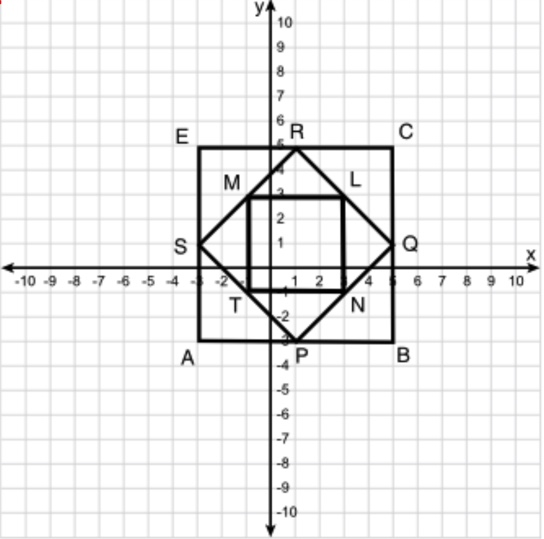
\includegraphics[width=0.9\columnwidth]{q24_figure}
  \caption{Graphic}
\end{figure}
\par
The information given to us is the following:
\begin{itemize}
  \item Points S, P, Q, and R are midpoints of ABCE
  \item T, N, L, and M are midpoints of PQRS
\end{itemize}
\newpage
Since we can already see the coordinates of M and L, we can calculate the slope between them, and use of them as a point which passes through the line to find the final equation of the line.
\begin{align}
  M = (-1, 3) \\
  L = (3, 3) \\
  m = \frac{3 - 3}{3 - (-1)} = 0
\end{align}
Since the slope is 0, this means that the equation has to be a horizontal line and since y values are always 3 regardless of what the x value is, we can deduce that the equation of ML is:
\begin{align}
  y = 3 
\end{align}
\end{center}
\end{document}
